\section{Sprint 6}\label{s6}
Im sechsten und letzten Sprint wurden diese beiden Stories bearbeitet:
\begin{itemize}
   \item Die Kommunikation mit den Stromzählern soll asynchron ausgeführt werden.
   \item SonarQube soll aufgesetzt werden und die gemeldete Fehler bearbeitet werden.
\end{itemize}
Neben diesen Stories wurde Zeit eingeplant, um bei den Nutzern der Anwendung ein letztes Mal ausführliches Feedback einzuholen.
Kleinere Änderungen und Bugfixes, welche aus dem Feedback hervorgehen, sollen ebenfalls direkt im Sprint umgesetzt werden.
Die folgenden Abschnitte geben Auskunft über die erwähnten Arbeiten.

\subsection{Asynchrone Kommunikation}
\dq Die Kommunikation mit den Stromzähler soll asynchron ausgeführt werden.\dq
\subsubsection{Ziele}
Bisher funktioniert die Kommunikation mit den Zählern so, dass diese direkt im UI Thread ausgeführt wird.
Dies hat den Nachteil, dass die Benutzerschnittstelle während der Kommunikation eingefroren ist und nicht auf weitere Eingaben des Benutzers reagiert.
Ein weiterer Nachteil der bisherigen Implementation ist, dass Kommunikationsfehler zu Abstürzen der ganzen Anwendung führen.
Das Ziel dieser Story ist es, die Kommunikation in einen Thread auszulagern und so asynchron auszuführen.
Dabei soll Wert auf die Fehlertoleranz der Implementation gelegt werden.


\subsubsection{Vorgehen \& Schwierigkeiten}\label{s6vorgehenasync}
In \ref{atsUmsetztung} wurde erklärt, wie der Code des \ac{ATS} eingebunden wurde.
Bisher war das Befehlsinterpreter Projekt eine direkte Abhängigkeit des DlmsQuickAccess.Dlms Projekts.
Die benötigten Klassen wurden dort instanziiert und verwendet. 
Dies führt dazu, dass DlmsQuickAccess.Dlms stark an den Befehlsinterpreter gekoppelt ist.
Ein Austausch des Kommunikationsstacks wäre mit grösseren Anpassungen verbunden.
Wie in Abschnitt \ref{portability} erklärt wurde, sind dies Anzeichen von tiefer Portabilität.

\begin{figure}[H]
   \centering
   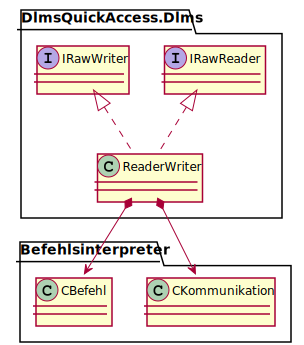
\includegraphics[width=0.5\textwidth]{gfx/dlms_vorher.png}
   \caption{
      Reduziertes Klassendiagramm um die ReaderWriter Klasse vor der Dependency Inversion
   }
   \label{fig:dlms_vorher}
\end{figure}

Da in diesem Sprint Änderungen am Kommunikationscode, also an DlmsQuickAccess.Dlms, geplant sind, wurde als erstes die zuvor genannte Kopplung bereinigt.
Dazu wurde das Dependency Inversion Principle angewendet.
Dieses besagt, dass High-Level-Module nicht von Low-Level-Modulen abhängen sollen.
Beide sollten von Abstraktionen abhängig sein \parencite{madasu35solid}.
Das Klassendiagramm in Abbildung \ref{fig:dlms_vorher} zeigt, wie die Klasse \textit{ReaderWriter} von Klassen des Befehlsinterpreter abhängig ist.
Wie die Abhängigkeiten nach dem Refactoring nach Dependency Inversion Principle aussehen, ist in Abblidung \ref{fig:dlms_nachher} gezeigt.
Mit dem \textit{ICommunicator} Interface definiert DlmsQuickAccess.Dlms nun lediglich die Schnittstelle eines Objekts, welches vom \textit{ReaderWriter} benötigt wird.
Dieses wird mit der \textit{Communicator} Klasse implementiert. Eine Instanz dieser Klasse kann nun in den \textit{ReaderWriter} injected werden.
Somit wurde die Koppelung von DlmsQuickAccess.Dlms und Befehlsinterpreter aufgelöst.


\begin{figure}[H]
   \centering
   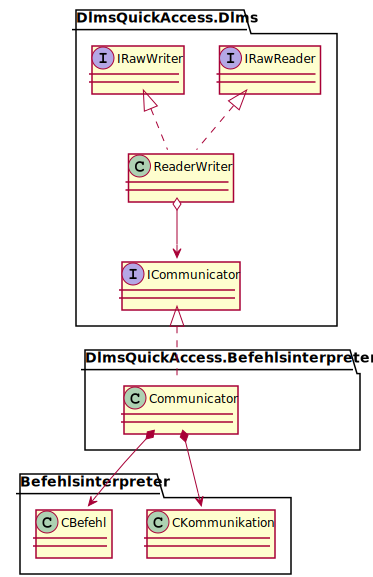
\includegraphics[width=0.5\textwidth]{gfx/dlms_nachher.png}
   \caption{
      Reduziertes und vereinfachtes Klassendiagramm um die ReaderWriter Klasse nach der Dependency Inversion
   }
   \label{fig:dlms_nachher}
\end{figure}

Die Asynchronität in der Kommunikation wurde mithilfe des \ac{TAP} umgesetzt.
Dies ist das von Microsoft empfohlene Pattern für die asynchrone Implementationen mit .NET \parencite{async}.
Das \ac{TAP} basiert auf der \textit{Task} Klasse, welche eine asynchron ausführte Operation repräsentiert.
Der Aufrufer einer asynchronen Methode erhält, noch bevor die asynchrone Operation gestartet wurde, ein \textit{Task} Objekt als Rückgabewert.
Dieses kann er beispielsweise dazu nutzen, um auf die Beendung der Operation synchron zu warten oder deren Status abzufragen.

Als der Code im DlmsQuickAccess.Dlms Projekt auf das \ac{TAP} Pattern umgeschrieben wurde, funktionierte die Kommunikation mit den Zählern nicht mehr.
Eine Fehlermeldung sagte, dass der COM-Port nicht geöffnet werden konnte.
Beim debuggen des \ac{ATS} Code stellte es sich heraus, dass dieser den Namen des aktuellen Threads nutzt, um seinen internen Zustand zu verwalten.
Dazu liest und schreibt er \textit{System.CurrentThread.Name}.
Bei \ac{TAP} werden die Operationen jeweils in Threads eines geteilten Pools ausgeführt, welche alle den gleichen Namen tragen.
Dieses Problem wurde so gelöst, dass im \ac{ATS} Code alle Referenzen zum Namen des aktuellen Threads auf eine Konstante geändert wurden.
Da beim DlmsQuickAccess nur eine Kommunikation mit einem Gerät vorgesehen ist, sollte dies kein Problem darstellen.


\subsection{SonarQube}\label{s6:sonar}
Im Abschnitt \ref{quality:sonar} wurde das Tool SonarQube erklärt und festgehalten, dass es von der Landis+Gyr als bevorzugtes Software-Qualitatssicherungstool evaluiert wurde.
Zum Zeitpunkt dieser Arbeit verfügte die Landis+Gyr noch über keine laufende Instanz von SonarQube.
Deshalb wurde eine solche lokal auf dem Rechner des Entwicklers aufgesetzt.
Dies hat den Nachteil, dass ein Aufbau, wie er in Abschnitt \ref{sonar:funktionsweise} beschrieben ist, nicht möglich ist.
Anstelle des \ac{CI} Servers muss der Build jeweils manuell ausgeführt und an die lokale SonarQube Instanz übermittelt werden.
Für dieses Projekt stellt dies kein Problem dar, da nur ein einzelner Entwickler am Code arbeitet.

\begin{figure}[H]
   \centering
   \includegraphics[width=1.0\textwidth]{gfx/SonarQubeOverallWithATS.png}
   \caption{
      Übersicht über den Bericht von SonarQube beim ersten ausführen.
   }
   \label{fig:sonarFistRunWithAts}
\end{figure}

Als die Scanners das erste Mal ausgeführt wurden, zeigte SonarQube ernüchternde Resultate.
In Abbildung \ref{fig:sonarFistRunWithAts} ist eine Übersicht über die SonarQube Berichte dargestellt.
Nebst der hohen Anzahl Bugs, Vulnerabilities und Code Smells sind auch die Bewertungen von SonarQube in den Bereichen Reliabilität und Sicherheit nicht zufriedenstellend.
Bei genauere Betrachtung der einzelnen Meldungen konnte jedoch festgestellt werde, dass ein grosser Teil ihren Ursprung im \ac{ATS} Code haben.
Die tiefe Qualität des \ac{ATS} Codes, welche bereits im ersten Sprint (Abschnitt \ref{atsUmsetztung}) angeprangert wurde, bestätigte sich so.

Um eine Beurteilung des eigentlichen Codes des DlmsQuickAccess zu erhalten, wurde in SonarQube ein zweites Projekt aufgesetzt, bei welchem der \ac{ATS} exkludiert wurde.
Die Berichte fielen nun bedeuten besser aus.
Da die verbleibende Anzahl Bugs und Vulnerabilities nun überschaubar war, wurden diese als Teil dieser Story behoben.
Eine Interpretation der finalen SonarQube Ergebnisse ist im Abschnitt \ref{evalQuality} zu finden.


\subsection{Rückmeldungen}
Während des ganzen Projekts und speziell in diesem letzten Sprint wurden Rückmeldungen der Nutzer eingeholt.
Wenn diese thematisch nahe an einer geplanten Story lagen, wurden diese jeweils im Rahmen derselben umgesetzt.
Folgende Arbeiten wurden aufgrund von Nutzerfeedback im sechsten Sprint gemacht:
\begin{itemize}
   \item Die aktuelle Version der Anwendung wird neu im Startfenster sowie in der Log-Datei angezeigt.
   \item Wenn die Applikationen das erste Mal gestartet wird, sind im Startfenster noch keine Konfigurationen aufgelistet.
Es wurde ein Text hinzugefügt, welcher dem Nutzer erklärt, wie er Konfigurationsdateien öffnen kan.
   \item Wird im verwendeten Object Model eine Class Description referenziert, welche für die Applikation unbekannt ist, so führte dies zu Abstürzen.
Diese Abstürze werden neu verhindert, indem eine leere Class Description als Platzhalter eingesetzt wird.
\end{itemize}
Weitere Rückmeldungen, welche noch nicht umgesetzt werden konnten, sind im nächsten Kapitel (\ref{eval}) aufgeführt.





% dotnet sonarscanner begin /k:"DlmsQuickAccess_NoATS" /d:sonar.host.url="http://localhost:9000"  /d:sonar.login="8568d95955df20f319cd05320e41bc4c8dac02f3"
% dotnet build DlmsQuickAccess_NoWinUI.sln
% dotnet sonarscanner end /d:sonar.login="8568d95955df20f319cd05320e41bc4c8dac02f3"

% \subsection{Feedback}
% Chakrit: 
% - Landingscreen ist leer, wenn zuvor noch kein Produkt gestartet wurde. // auch von christoph
%    - Wo finde ich einen Browser? // Chistoph
% - Version nicht sichtbar im Loadingscreen
% - Version nicht sichtbar im Log
% - Wenn er via Windows startet steht im Log ein fehler.
% - Enter to search

% Someone:
% - Lesen von Arrays stimmt nicht richtig
%    - repro: Object list lesen

% Christoph:
% - Favoriten sind für mich eine Killerfeature
% - Klartext der Enums auch ein Killerfeature

% - Länge der Namen zu lang
% - Cursor in Suchfeld nicht gut sichtbar
% - Enter um Suche zu starten
% - Feedback, dass kommunikation im Gange ist
% - Feedback, wenn kommunikation fehlschlägt
% - CHOICE type nicht supported
% - Integers need to be correct length (leading 0)

% DMT2 QuickAccess verwende ich nur noch, wenn bei einzelnen Attribtue/Objekte die im DlmsQuickAccess nicht richtig funktionieren.
%    Wünsche mir, dass die Applikation weiterentwickelt wird und von der Firma den nötigen Support erhält.



% Ronny:
% - Eines wäre praktisch, wenn genesene Werte als Datei gespeichert werden könnten. Z.B. Yaml.
% - Bug, dass app crasht, wenn Description nicht vorhanden
% - Beim Auslesen von Arrays mit vielen Einträgen wird das UI schnell unübersichtlich.

% - Starten der Anwendung sehr Praktisch. Suchen in Windows nach "DlmsQuickAccess", Click auf das gewünschte Produkt und schon ist alles einsatzbereit.
% Beim DMT2 wusste man nie, welche Konfiguration gerade geladen war und das ändern dieser ist jeweils umständlich.
% - Die Schreib und Lesegeschwindigkeit ist eindrücklich.
